\documentclass[aspectratio=169,10pt]{beamer}

% ---- Encoding & fonts -----------------------------------------
\usepackage[utf8]{inputenc}
\usepackage[T1]{fontenc}
\usepackage{lmodern}                % fixes OMS/cmtt undefined glyphs

% ---- Theme ----------------------------------------------------
\usetheme{Madrid}
\usecolortheme{default}
\setbeamertemplate{navigation symbols}{}
\setbeamertemplate{footline}[frame number]

% ---- Packages -------------------------------------------------
\usepackage{booktabs}              % \toprule, \midrule, \bottomrule
\usepackage{listings}
\usepackage{xcolor}
\usepackage{tikz}
\usetikzlibrary{arrows.meta, positioning, shapes.geometric}
\usepackage{hyperref}

% ---- Colors ---------------------------------------------------
\definecolor{codebg}{RGB}{245,245,248}
\definecolor{codekw}{RGB}{0,90,180}
\definecolor{codestr}{RGB}{160,50,50}
\definecolor{codered}{RGB}{180,30,30}
\definecolor{codegreen}{RGB}{30,120,60}
\definecolor{panelblue}{RGB}{40,90,160}
\definecolor{panelred}{RGB}{170,40,40}
\definecolor{panelgreen}{RGB}{40,130,70}
\definecolor{panelgray}{RGB}{90,90,90}

% ---- Listings (ASCII-safe, no Unicode) ------------------------
\lstdefinestyle{code}{
  basicstyle=\ttfamily\scriptsize,
  backgroundcolor=\color{codebg},
  keywordstyle=\color{codekw}\bfseries,
  stringstyle=\color{codestr},
  commentstyle=\color{codegreen}\itshape,
  numbers=none,
  frame=single,
  rulecolor=\color{gray!40},
  breaklines=true,
  columns=fullflexible,
  keepspaces=true,
  showstringspaces=false,
  extendedchars=false,
  upquote=true,
}
\lstset{style=code}

% ---- Title (no math in \title -> no hyperref warning) ---------
\title{Secure SQL AI Agent}
\subtitle{Plain-English database queries, enforced by three independent security layers}
\author{Your Name}
\institute{Your Organisation}
\date{\today}

\begin{document}

% ===============================================================
\begin{frame}
  \titlepage
\end{frame}

% ===============================================================
\begin{frame}{The problem}
  \begin{block}{Users want to ask questions in English}
    \emph{``Show me the top 3 customers by revenue.''}\\
    \emph{``Cancel order ORD-2024-0011.''}\\
    \emph{``Which products have never been ordered?''}
  \end{block}

  \begin{alertblock}{Naive LLM-to-SQL is dangerous}
    \begin{itemize}
      \item LLM can emit \texttt{DROP TABLE users}
      \item LLM can be prompt-injected by malicious data
      \item An innocent question can hide \texttt{UPDATE} or \texttt{DELETE}
      \item Regex checks are bypassable; SQL is a full programming language
    \end{itemize}
  \end{alertblock}
\end{frame}

% ===============================================================
\begin{frame}{The solution: three independent security layers}
  \begin{columns}[T]
    \begin{column}{0.32\textwidth}
      \begin{block}{\centering Layer 1}
        \centering\textbf{Static validation}\\[2pt]
        \footnotesize AST parse $\rightarrow$ classify\\
        schema check $\rightarrow$ EXPLAIN
      \end{block}
    \end{column}
    \begin{column}{0.32\textwidth}
      \begin{block}{\centering Layer 2}
        \centering\textbf{Human approval}\\[2pt]
        \footnotesize Every write shown to\\
        the user before execution
      \end{block}
    \end{column}
    \begin{column}{0.32\textwidth}
      \begin{block}{\centering Layer 3}
        \centering\textbf{DB permissions}\\[2pt]
        \footnotesize Read role vs write role\\
        enforced by PostgreSQL
      \end{block}
    \end{column}
  \end{columns}

  \vspace{6pt}
  \begin{alertblock}{Design principle}
    No single layer is trusted. Each is independently sufficient to stop an unsafe write.
  \end{alertblock}
\end{frame}

% ===============================================================
\begin{frame}{Architecture}
  \centering
  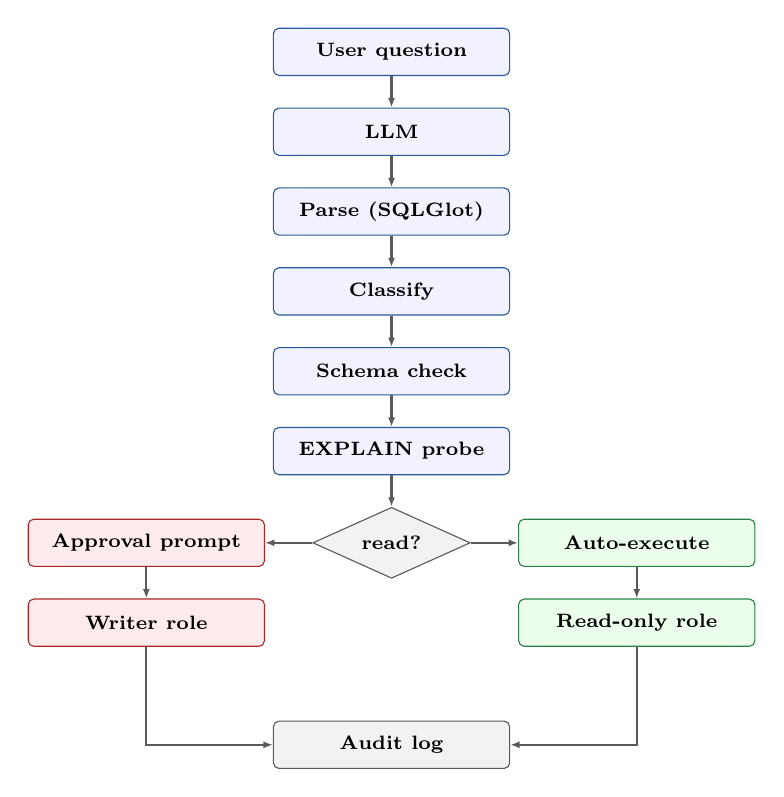
\begin{tikzpicture}[
    node distance=4mm,
    box/.style={rectangle, rounded corners=2pt, draw=panelblue, fill=blue!5,
                minimum width=3.0cm, minimum height=6mm, font=\scriptsize\bfseries, align=center},
    decnode/.style={diamond, aspect=2, draw=panelgray, fill=gray!10,
                    minimum width=2.0cm, minimum height=8mm, font=\scriptsize\bfseries, align=center},
    arrow/.style={-{Latex[length=1.2mm]}, draw=panelgray, thick},
    lab/.style={font=\scriptsize\itshape, text=panelgray},
  ]
    \node[box] (user)    {User question};
    \node[box, below=of user]   (llm)  {LLM};
    \node[box, below=of llm]    (parse){Parse (SQLGlot)};
    \node[box, below=of parse]  (class){Classify};
    \node[box, below=of class]  (schema){Schema check};
    \node[box, below=of schema] (explain){EXPLAIN probe};
    \node[decnode, below=of explain] (dec){read?};

    \node[box, right=6mm of dec, fill=green!8, draw=panelgreen] (auto)  {Auto-execute};
    \node[box, below=of auto,    fill=green!8, draw=panelgreen] (roro)  {Read-only role};

    \node[box, left=6mm of dec,  fill=red!8,  draw=panelred]   (appr)  {Approval prompt};
    \node[box, below=of appr,    fill=red!8,  draw=panelred]   (wrol)  {Writer role};

    \node[box, below=18mm of dec, fill=gray!10, draw=panelgray] (audit) {Audit log};

    \foreach \a/\b in {user/llm, llm/parse, parse/class, class/schema, schema/explain, explain/dec}
      \draw[arrow] (\a) -- (\b);

    \draw[arrow] (dec.east)  -- (auto.west);
    \draw[arrow] (dec.west)  -- (appr.east);
    \draw[arrow] (auto) -- (roro);
    \draw[arrow] (appr) -- (wrol);

    \draw[arrow] (roro.south) |- (audit.east);
    \draw[arrow] (wrol.south) |- (audit.west);
  \end{tikzpicture}

  \vspace{4pt}
  {\footnotesize LLM is \emph{untrusted input}. Everything after it is deterministic Python.}
\end{frame}

% ===============================================================
\begin{frame}[fragile]{Layer 1: AST classification}
  \begin{lstlisting}[language=Python]
class SQLClassifier:
    def classify(self, tree):
        if isinstance(tree, exp.Select):     # read?
            if tree.find(exp.Into):          # SELECT INTO -> reject
                return unsupported("SELECT INTO")
            if tree.find(exp.Lock):          # FOR UPDATE -> reject
                return unsupported("FOR UPDATE")
            for fn in dangerous_functions(tree):  # pg_read_file, dblink
                return unsupported(fn)
            return read()
        if isinstance(tree, (exp.Update, exp.Delete, exp.Insert)):
            return write()
        if isinstance(tree, (exp.Create, exp.Drop, exp.Alter)):
            return ddl() if ENABLE_DDL else unsupported("DDL disabled")
        return unsupported("unknown")
  \end{lstlisting}

  \begin{block}{Explicitly rejected regardless of class}
    \footnotesize
    Multiple statements \textperiodcentered{} SELECT INTO \textperiodcentered{}
    FOR UPDATE \textperiodcentered{} data-modifying CTEs \textperiodcentered{}
    EXPLAIN ANALYZE \textperiodcentered{} unapproved functions \textperiodcentered{}
    UPDATE/DELETE without WHERE
  \end{block}
\end{frame}

% ===============================================================
\begin{frame}[fragile]{Layer 2: one-time approval tokens}
  \begin{lstlisting}[language=Python]
def create_token(request):
    token = secrets.token_urlsafe(32)
    self._pending[token] = ApprovalToken(
        token=token,
        sql_hash=sha256(request.sql),
        params_hash=sha256(json.dumps(request.parameters, sort_keys=True)),
    )
    return token

def verify_and_consume(token, sql, params):
    stored = self._pending.pop(token, None)          # one-time
    if stored is None:
        raise ApprovalError("token invalid or already used")
    if stored.sql_hash != sha256(sql):
        raise ApprovalError("token not bound to this SQL")
    if stored.params_hash != sha256(json.dumps(params, sort_keys=True)):
        raise ApprovalError("token not bound to these parameters")
  \end{lstlisting}

  \begin{alertblock}{Editing at the prompt is safe}
    Edited SQL is re-parsed, re-classified, re-validated, and the user sees a
    \emph{fresh} approval prompt. Old tokens are invalidated on use.
  \end{alertblock}
\end{frame}

% ===============================================================
\begin{frame}[fragile]{Layer 3: database-enforced permissions}
  \begin{columns}[T]
    \begin{column}{0.5\textwidth}
      \begin{block}{\footnotesize Read-only role}
        \begin{lstlisting}[language=SQL]
GRANT SELECT
  ON ALL TABLES IN SCHEMA public
  TO sql_agent_readonly;
-- no INSERT/UPDATE/DELETE
        \end{lstlisting}
      \end{block}
    \end{column}
    \begin{column}{0.5\textwidth}
      \begin{block}{\footnotesize Writer role}
        \begin{lstlisting}[language=SQL]
GRANT SELECT, INSERT, UPDATE, DELETE
  ON ALL TABLES IN SCHEMA public
  TO sql_agent_writer;
-- no DDL, no superuser
        \end{lstlisting}
      \end{block}
    \end{column}
  \end{columns}

  \vspace{6pt}
  \begin{alertblock}{The critical test}
    \footnotesize
    \texttt{psql -U sql\_agent\_readonly -c "INSERT INTO products ..."} \\
    \texttt{ERROR: permission denied for table products}
  \end{alertblock}

  \centering\footnotesize
  Even if all Python were bypassed, PostgreSQL itself refuses the write.
\end{frame}

% ===============================================================
\begin{frame}[fragile]{The full pipeline (one read request)}
  \begin{lstlisting}
You: list customers with more than one order

Generated SQL:
  SELECT c.id, c.name, c.email
  FROM customers c JOIN orders o ON c.id = o.customer_id
  GROUP BY c.id, c.name, c.email
  HAVING COUNT(o.id) > 1;

Validation: [PASS] schema

Result: 1 row(s) returned.
  {"id": 1, "name": "Alice Johnson", "email": "alice@example.com"}
  \end{lstlisting}

  \begin{block}{What happened behind the scenes}
    \footnotesize
    LLM generated SQL $\rightarrow$ SQLGlot parsed it $\rightarrow$
    classified as read $\rightarrow$ every column resolved against live schema
    $\rightarrow$ \texttt{EXPLAIN} succeeded on read-only connection
    $\rightarrow$ executed $\rightarrow$ audited
  \end{block}
\end{frame}

% ===============================================================
\begin{frame}[fragile]{The full pipeline (one write request)}
  \begin{lstlisting}
You: change the price of product 1 to 1299

==========================================
          WRITE APPROVAL REQUIRED
==========================================
Operation: UPDATE
SQL:
  UPDATE products SET price = :price WHERE id = :product_id;
Parameters:
  price = 1299
  product_id = 1
Tables: products
Description:
  Update the price of product 1 to 1299.
1. Approve   2. Reject   3. Edit
==========================================
Approve? (yes/no/edit): yes

Affected rows: 1
  \end{lstlisting}

  \centering\footnotesize No approval? No execution. Ever.
\end{frame}

% ===============================================================
\begin{frame}[fragile]{Bounded self-repair}
  \begin{lstlisting}
You: show the age of each customer

[attempt 1] LLM: SELECT name, age FROM customers
            validator: Column 'age' does not exist

[attempt 2] LLM (with error fed back):
            SELECT name, created_at FROM customers
            validator: PASS

Result: 2 row(s) returned.

(If attempts exceeded: status=validation_failed, nothing executes.)
  \end{lstlisting}

  \begin{alertblock}{Hard limits}
    \footnotesize
    \texttt{MAX\_SQL\_REPAIR\_ATTEMPTS=2} \textperiodcentered{}
    no bypass of validation during repair \textperiodcentered{}
    no read-to-write upgrades without full approval flow
  \end{alertblock}
\end{frame}

% ===============================================================
\begin{frame}{Live demo}
  \begin{block}{Reads (execute automatically)}
    \begin{itemize}
      \item ``top 3 customers by total revenue''
      \item ``which products have never been ordered''
      \item ``average rating per category''
      \item ``orders created in the last 30 days that are still pending''
    \end{itemize}
  \end{block}

  \begin{block}{Writes (approval required)}
    \begin{itemize}
      \item ``change the price of product 1 to 1299''
      \item ``cancel order ORD-2024-0011''
      \item ``delete the review by customer 4 for product 6''
    \end{itemize}
  \end{block}

  \begin{alertblock}{Rejections (deterministic)}
    \begin{itemize}
      \item ``drop table customers'' $\rightarrow$ DDL disabled
      \item ``delete all orders'' $\rightarrow$ UPDATE/DELETE without WHERE
      \item ``select * from users; drop table users'' $\rightarrow$ multi-statement
    \end{itemize}
  \end{alertblock}
\end{frame}

% ===============================================================
\begin{frame}{Stack and scale}
  \begin{columns}[T]
    \begin{column}{0.5\textwidth}
      \begin{block}{Technology}
        \footnotesize
        \begin{tabular}{@{}ll@{}}
          \toprule
          \textbf{Layer} & \textbf{Tool} \\
          \midrule
          Language  & Python 3.11+ \\
          Database  & PostgreSQL 17/18 \\
          DB access & SQLAlchemy 2 + Psycopg 3 \\
          SQL parse & SQLGlot \\
          Config    & Pydantic 2 \\
          LLM       & Ollama (local) \\
          LLM alt   & OpenAI \\
          Tests     & pytest \\
          Packaging & Docker + Compose \\
          \bottomrule
        \end{tabular}
      \end{block}
    \end{column}
    \begin{column}{0.5\textwidth}
      \begin{block}{Project numbers}
        \footnotesize
        \begin{tabular}{@{}lr@{}}
          \toprule
          \textbf{Metric} & \textbf{Value} \\
          \midrule
          Python modules      & 20 \\
          Unit tests          & 41 \\
          Security layers     & 3 \\
          LLM providers       & 2 built-in \\
          DDL paths           & 1 (opt-in) \\
          Lines of agent code & $\sim$350 \\
          \bottomrule
        \end{tabular}
      \end{block}
    \end{column}
  \end{columns}
\end{frame}

% ===============================================================
\begin{frame}{Results and guarantees}
  \begin{block}{What the system guarantees}
    \begin{itemize}
      \item \textbf{Reads} always execute on a connection that \emph{cannot} write
      \item \textbf{Writes} never execute without a one-time approval bound to
            the exact SQL and parameters
      \item \textbf{Unsupported SQL} is rejected by explicit allowlist, not by
            blocklist guesswork
      \item \textbf{Every request} is written to a structured audit log
      \item \textbf{Failure is fail-closed} — uncertainty means rejection
    \end{itemize}
  \end{block}

  \begin{alertblock}{What it does \emph{not} guarantee}
    \begin{itemize}
      \item A query that passes \texttt{EXPLAIN} can still fail at runtime
            (constraints, triggers, races) — the transaction is rolled back
      \item The LLM's output is not trustable; only the pipeline is
    \end{itemize}
  \end{alertblock}
\end{frame}

% ===============================================================
\begin{frame}{Known limitations}
  \begin{itemize}
    \item Live validation is \emph{best-effort} — \texttt{EXPLAIN} does not
          catch every runtime error
    \item Write-path schema validation is conservative by design
          (fail-closed over permissive)
    \item Local LLM quality varies with model size — smaller models produce
          less clean SQL but the pipeline stays safe
    \item One database per agent instance
    \item DDL support exists but is off by default
  \end{itemize}
\end{frame}

% ===============================================================
\begin{frame}{Extending the project}
  \begin{block}{Add a new LLM provider}
    \footnotesize
    Implement \texttt{LLMClient.generate\_sql()} in $\sim$40 lines; wire one
    branch in \texttt{main.py}. Parser, validators, approval, executor, and
    audit are unchanged.
  \end{block}

  \begin{block}{Add a REST or web interface}
    \footnotesize
    Wrap \texttt{QueryService.execute(request, user) -> AgentResponse} in FastAPI.
    Replace \texttt{CLIApprovalProvider} with a Slack/email/WebSocket provider
    implementing the same protocol.
  \end{block}

  \begin{block}{Add another SQL dialect}
    \footnotesize
    Change \texttt{DATABASE\_DIALECT} in \texttt{.env}. Add a dialect-specific
    \texttt{LiveValidator} for the new database's non-executing plan probe.
  \end{block}
\end{frame}

% ===============================================================
\begin{frame}{Summary}
  \begin{block}{What we built}
    A production-oriented SQL agent that lets non-technical users query a
    database in plain English, with \textbf{three independent security layers}
    that make unsafe writes structurally impossible.
  \end{block}

  \begin{block}{Why it works}
    \begin{itemize}
      \item Deterministic Python classifies and validates every query
      \item Humans approve every write, bound to exact SQL and parameters
      \item PostgreSQL roles enforce the last line of defense
    \end{itemize}
  \end{block}

  \centering\Large\bfseries Questions?
\end{frame}

\end{document}
